\documentclass[journal,12pt,twocolumn]{IEEEtran}

\usepackage{setspace}
\usepackage{gensymb}
\singlespacing
\usepackage[cmex10]{amsmath}

\usepackage{amsthm}

\usepackage{mathrsfs}
\usepackage{txfonts}
\usepackage{amsmath}
\usepackage{stfloats}
\usepackage{float}
\usepackage{bm}
\usepackage{tikz}
\usepackage{pgfplots}
\pgfplotsset{compat=1.7}
\usepackage{cite}
\usepackage{cases}
\usepackage{subfig}

\usepackage{longtable}
\usepackage{multirow}

\usepackage{enumitem}
\usepackage{mathtools}
\usepackage{steinmetz}
\usepackage{tikz}
\usepackage{circuitikz}
\usepackage{verbatim}
\usepackage{tfrupee}
\usepackage[breaklinks=true]{hyperref}
\usepackage{graphicx}
\usepackage{tkz-euclide}

\usetikzlibrary{calc,math}
\usetikzlibrary{shapes.geometric, arrows}
\usepackage{listings}
    \usepackage{color}                                            %%
    \usepackage{array}                                            %%
    \usepackage{longtable}                                        %%
    \usepackage{calc}                                             %%
    \usepackage{multirow}                                         %%
    \usepackage{hhline}                                           %%
    \usepackage{ifthen}                                           %%
    \usepackage{lscape}
\usepackage{multicol}
\usepackage{chngcntr}
\usepackage{hyperref}
\hypersetup{
    colorlinks=true,
    linkcolor=blue,
    filecolor=blue,
    urlcolor=blue,
}
\DeclareMathOperator*{\Res}{Res}
\DeclareMathOperator{\sinc}{sinc}
\DeclareMathOperator{\Sa}{Sa}
\DeclareMathOperator{\rect}{rect}

\renewcommand\thesection{\arabic{section}}
\renewcommand\thesubsection{\thesection.\arabic{subsection}}
\renewcommand\thesubsubsection{\thesubsection.\arabic{subsubsection}}



\hyphenation{optical networks semiconduc-tor}
\def\inputGnumericTable{}                                 %%

\lstset{
%language=C,
frame=single, 
breaklines=true,
columns=fullflexible
}
\date{March 2021}

\makeatletter
\setlength{\@fptop}{0pt}
\makeatother

\begin{document}

\newtheorem{theorem}{Theorem}[section]
\newtheorem{problem}{Problem}
\newtheorem{proposition}{Proposition}[section]
\newtheorem{lemma}{Lemma}[section]
\newtheorem{corollary}[theorem]{Corollary}
\newtheorem{example}{Example}[section]
\newtheorem{definition}[problem]{Definition}

\newcommand{\BEQA}{\begin{eqnarray}}
\newcommand{\EEQA}{\end{eqnarray}}
\newcommand{\define}{\stackrel{\triangle}{=}}
\bibliographystyle{IEEEtran}
\raggedbottom
\setlength{\parindent}{0pt}
\providecommand{\mbf}{\mathbf}
\providecommand{\pr}[1]{\ensuremath{\Pr\left(#1\right)}}
\providecommand{\qfunc}[1]{\ensuremath{Q\left(#1\right)}}
\providecommand{\fn}[1]{\ensuremath{f\left({#1}\right)}}
\providecommand{\e}[1]{\ensuremath{E\left(#1\right)}}
\providecommand{\sbrak}[1]{\ensuremath{{}\left[#1\right]}}
\providecommand{\lsbrak}[1]{\ensuremath{{}\left[#1\right.}}
\providecommand{\rsbrak}[1]{\ensuremath{{}\left.#1\right]}}
\providecommand{\brak}[1]{\ensuremath{\left(#1\right)}}
\providecommand{\lbrak}[1]{\ensuremath{\left(#1\right.}}
\providecommand{\rbrak}[1]{\ensuremath{\left.#1\right)}}
\providecommand{\cbrak}[1]{\ensuremath{\left\{#1\right\}}}
\providecommand{\lcbrak}[1]{\ensuremath{\left\{#1\right.}}
\providecommand{\rcbrak}[1]{\ensuremath{\left.#1\right\}}}
\theoremstyle{remark}
\newtheorem{rem}{Remark}
\newcommand{\sgn}{\mathop{\mathrm{sgn}}}
\newcommand{\comb}[2]{{}^{#1}\mathrm{C}_{#2}}
\providecommand{\abs}[1]{\vert#1\vert}
\providecommand{\res}[1]{\Res\displaylimits_{#1}} 
\providecommand{\norm}[1]{\lVert#1\rVert}
%\providecommand{\norm}[1]{\lVert#1\rVert}
\providecommand{\mtx}[1]{\mathbf{#1}}
\providecommand{\mean}[1]{E\sbrak{ #1 }}
\providecommand{\fourier}{\overset{\mathcal{F}}{ \rightleftharpoons}}
%\providecommand{\hilbert}{\overset{\mathcal{H}}{ \rightleftharpoons}}
\providecommand{\system}{\overset{\mathcal{H}}{ \longleftrightarrow}}
\providecommand{\ztrans}{\overset{\mathcal{Z}}{ \rightleftharpoons}}
	%\newcommand{\solution}[2]{\textbf{Solution:}{#1}}
\newcommand{\solution}{\noindent \textbf{Solution: }}
\newcommand{\cosec}{\,\text{cosec}\,}
\providecommand{\dec}[2]{\ensuremath{\overset{#1}{\underset{#2}{\gtrless}}}}
\newcommand{\myvec}[1]{\ensuremath{\begin{pmatrix}#1\end{pmatrix}}}
\newcommand{\mydet}[1]{\ensuremath{\begin{vmatrix}#1\end{vmatrix}}}
\numberwithin{equation}{subsection}
\makeatletter
\@addtoreset{figure}{problem}
\makeatother
\let\StandardTheFigure\thefigure
\let\vec\mathbf

\vspace{3cm}
\title{Quiz2}
\author{Adhvik Mani Sai Murarisetty - AI20BTECH11015}
\maketitle
\newpage
\bigskip
\renewcommand{\thetable}{\theenumi}

Download latex-tikz codes from 
%
\begin{lstlisting}
https://github.com/adhvik24/EE3900/blob/main/quiz2/main.tex
\end{lstlisting}
%
Download python codes from 
%
\begin{lstlisting}
https://github.com/adhvik24/EE3900/blob/main/quiz2/code.py
\end{lstlisting}
\section*{Problem 3.7 (a)}
\textbf{3.7 (a)}  The input to a casual linear time-invariant system is
\begin{align}
    x[n]=u[-n-1]+\brak{\frac{1}{2}}^n u[n]
\end{align}
The z-transform of the output of this system is
\begin{align}
    Y(z)=\frac{-\frac{1}{2}z^{-1}}{\brak{1-\frac{1}{2}z^{-1}}\brak{1+z^{-1}}}
\end{align}
\begin{enumerate}[label=(\alph*)]
    \item Determine H(z), the z-transform of the system impulse response. Be sure to specify the region of convergence.
    \item What is the region of convergence for Y(z).
    \item Determine y[n].
\end{enumerate}
\section*{Solution 3.7(a)}
\begin{definition}
We say that a system is \textbf{Causal} if the output of a system at a given time instance is independent of the future input values, i.e the output at a particular instance only depends on the present and past input values.
\end{definition}
\begin{lemma}
A system is causal if and only if the transfer function $h[n]$ satisfies $h[n] = 0 , n<0$
\end{lemma}
\begin{proof}
Let the input signal be given by $x[n]$ and the output signal be given by $y[n]$, then, we know in an LTI system:
\begin{align}
    y[n] = h[n] * x[n] = \sum_{k = -\infty}^\infty h[k]x[n-k]
\end{align}
Since, $y[n]$ is causal, it should be independent of future values of $n$. \\
If $k < 0$, then $n - k > n$, which is undesirable, and thus, to keep $y[n]$ independent of future values, $h[k] = 0 , k< 0$
\end{proof}
\begin{lemma}
A system is said to be causal if and only if the ROC of the impulse function lies outside the outermost pole.
\label{Causal}
\end{lemma}

\begin{lemma}
If $x[n] = a^nu[n]$, where 
\begin{align}
    u[n] = 
    \begin{cases}
    1 & n \geq 0\\
    0 & otherwise
    \end{cases}
\end{align}
then $x[n] \ztrans X[z] = \frac{1}{1 - az^{-1}}$ with ROC = $\abs{z}>a$
\label{0}
\end{lemma}
\begin{proof}
Using the formula for the sum of an infinite GP, we get:
\begin{align}
    x[n] = 
    \begin{cases}
    a^n & n\geq 0\\
    0 & otherwise
    \end{cases}\\
    \mathcal{Z}\{x[n]\} = X[z] = \sum_{n = -\infty}^\infty x[n]z^{-n}\\
    = \sum_{n = -\infty}^0 0 \times z^{-n} + \sum_{n = 0}^{\infty} (az^{-1})^n\\
     = \frac{1}{1 - az^{-1}} , ROC = \abs{az^{-1}} < 1\\
      = \frac{1}{1 - az^{-1}} , ROC =  \abs{z} > a
\end{align}
\end{proof}
\begin{lemma}
If $x[n] = -a^nu[-n-1]$, then $x[n] \ztrans X[z] = \frac{1}{1 - az^{-1}}$ with ROC = $\abs{z}<a$ 
\label{1}
\end{lemma}
\begin{proof}
Using the formula for the sum of an infinite GP, we get:

\begin{align}
    x[n] &= 
    \begin{cases}
    -a^n & n\leq -1\\
    0 & otherwise
    \end{cases}
\end{align}
\begin{align}
   \nonumber \mathcal{Z}\{x[n]\} &= X[z] = \sum_{n = -\infty}^\infty x[n]z^{-n}\\
  \nonumber  &= \sum_{n = -\infty}^\infty \cbrak{-a^nu[-n-1]}z^{-n}\\
  \nonumber    &= \sum_{n = -\infty}^{-1} {-a^n}z^{-n} + \sum_{n = -1}^{\infty} 0\times z^{-1}\\
  \nonumber  &=-\sum_{n = 1}^{\infty} (a^{-1}z)^n =1-\sum_{n = 0}^{\infty} (a^{-1}z)^n\\
  \nonumber   &= 1-\frac{1}{1 - a^{-1}z} , ROC = \abs{a^{-1}z} < 1\\
     X[z] &= \frac{1}{1 - az^{-1}} , ROC =  \abs{z} < a
\end{align}
\end{proof}

We are given x[n] as,
\begin{align}
    x[n]=u[-n-1]+\brak{\frac{1}{2}}^n u[n]
\end{align}
Then the z-transform of x[n] using \eqref{0} and \eqref{1} is,
\begin{align}
    X(z)=\frac{-1}{1-z^{-1}}+\frac{1}{1-\frac{1}{2}z^{-1}},\frac{1}{2}<\abs{z}<1\label{2}
\end{align}
We know that H(z) is,
\begin{align}
    H(z)=\frac{Y(z)}{X(z)}\label{3}
\end{align}
Using Y(z) and \eqref{2} in \eqref{3}, will result in H(z) as,
\begin{align}
    H(z)&=\frac{Y(z)}{X(z)}=\frac{\frac{-\frac{1}{2}z^{-1}}{\brak{1-\frac{1}{2}z^{-1}}\brak{1+z^{-1}}}}{\frac{-1}{1-z^{-1}}+\frac{1}{1-\frac{1}{2}z^{-1}}}\\
  \nonumber  &=\frac{-\frac{1}{2}z^{-1}}{\brak{1-\frac{1}{2}z^{-1}}\brak{1+z^{-1}}}.\frac{\brak{1-\frac{1}{2}z^{-1}}\brak{1-z^{-1}}}{-\frac{1}{2}z^{-1}}\\
  \nonumber H(z)&= \frac{\brak{1-z^{-1}}}{\brak{1+z^{-1}}}\\
  H(z)&=\frac{{2}}{\brak{1+z^{-1}}}-1
\end{align}
From the above decomposition, we find that the poles of $H(z)$ are $z = -1$, and the zeroes are $z = 1$, as shown in the plot-zero diagram given below.
Thus, we can also say the outermost pole is $z = -1$, and thus, from \eqref{Causal}, As given the system is casual, that implies \textbf{ROC is $\abs{z} > 1$.}

\begin{figure}[!htp]
    \centering
    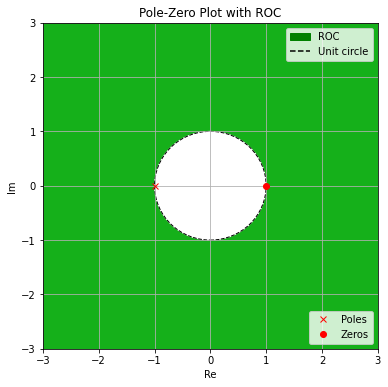
\includegraphics[width=\columnwidth]{1.png}
    \caption{Pole-Zero plot for $H(z)$ }
    \label{f0}
\end{figure}

$\therefore$ Z transform of the system impulse response is $H(z)=\frac{\brak{1-z^{-1}}}{\brak{1+z^{-1}}}$ and the ROC is $abs{z} > 1$
\end{document}
